\newpage
\section{Informationen vom Thesis-Day} \label{infos}
Siehe auch Wissenschaftliches Arbeiten~\footcite[\vglf][S. 1]{Balzert.2008}. %ohne textcommands
Damit sollten alle wichtigen Informationen abgedeckt sein ;-)~\footcite[\vglf][\pagef 1]{Balzert.2008} %mit textcommands
Hier gibt es noch ein Beispiel für ein direktes Zitat\footcite[][\pagef 1]{Balzert.2008} %mit textcommands

\subsection{Pre-Anmeldephase}
\subsubsection{Vorüberlegungen}
Trichtermethode: Man beginnt mit der eigentlichen  Konklusion und überlegt dann, welche allgemeinen Teile dafür benötigt werden.

Welchen Mehrwert soll die Arbeit bieten \footnote{Diese Fu\ss note hat inhaltlich keinen Sinn. Es soll nur ein langer Text generiert werden, dass dieser Vermerk über zwei Zeilen reicht und bündig dargestellt wird.}? Auch darüber nachdenken, wie die Arbeit einen selbst weiter bringen kann. Studienverlauf prüfen. Welche Vorlesungen hat mich besonders interessiert? Wo liegen meine Stärken etc.

\begin{enumerate}
\item Themenfindung
\item Literaturrecherche
\item Gliederung/Motivationspapier erstellen
\item Betreuerauswahl (siehe Liste im \ac{OC})
\item Anmeldung (ab 141 Credits möglich)
\end{enumerate}

\subsubsection{Anregungen finden}
\begin{itemize}
\item \href{http://www.diplom.de}{www.diplom.de}
\item \href{http://www.hausarbeiten.de}{www.hausarbeiten.de}
\item Datenbanken aus Tools and Methods
\item etc.
\end{itemize}

\newpage
\subsection{Anfertigungsphase}
Die Anmeldung ist mittlerweile jeden Mittwoch möglich.
\begin{figure}[H]
\caption{FOM-Vorgaben zur Thesis im Online-Campus}
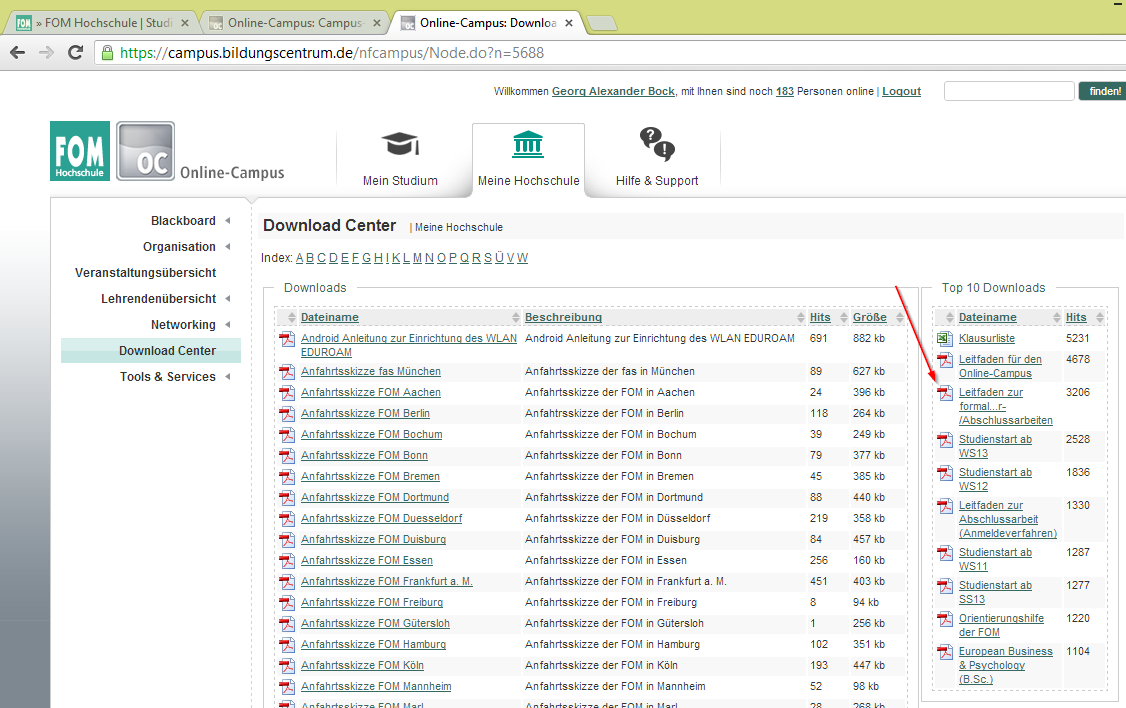
\includegraphics[width=0.9\textwidth]{campusDownload}
\\
\cite[Quelle: Vgl.][]{FOM}
\end{figure}

Laut Herrn Keller sollte der Umfang der Thesis (für eine gute Note) eher im Bereich der 60 Seiten liegen. Wie immer ist das vermutlich mit dem Betreuer abzustimmen. Die Liste der Dozenten, die Abschlussarbeiten betreuen, findet sich auch im \ac{OC}.

Zeit zur Erstellung der Thesis 2-4 Monate.

Es müssen zwei gedruckte Arbeiten abgegeben werden. Flüchtige Quellen als PDF ausgeben lassen und auf CD abgeben. Thesis zusätzlich digital einreichen. Beim Binden der Thesis auf Qualität achten. Haptik und erster Eindruck sind in der Bewertung \enquote{auch} wichtig. Arbeiten können in jedem FOM Studienzentrum abgegeben werden.

\subsection{Post-Abgabephase}
Nach Abgabe ca. 2 Wochen bis zum Kolloquium.

Kolloquium:
\begin{itemize}
\item Dauer: 30 Minuten
\item Präsentation (manche Prüfer wollen eine, andere nicht)
\item Betreuer vorher fragen was er möchte
\item Es gibt einen Frageteil, dieser bezieht sich auf die Arbeit, kann aber auch darüber hinaus gehen.
\item Der Tag des Kolloquiums steht auf der Endbenotung
\item Thesis und Kolloquium sind zwei getrennte Prüfungsbereiche. Für beide gibt es nur zwei Versuche.
\item Am Tag des Kolloquiums erhält man die Bestätigung, ob bestanden oder nicht
\end{itemize}
